%--------------------------------------
% Create title frame
\titleframe


%==============================================
% \section*{Introduction}
%==============================================
\begin{frame}{\large \textbf{Introduction}}

  \begin{minipage}{8.2cm}
    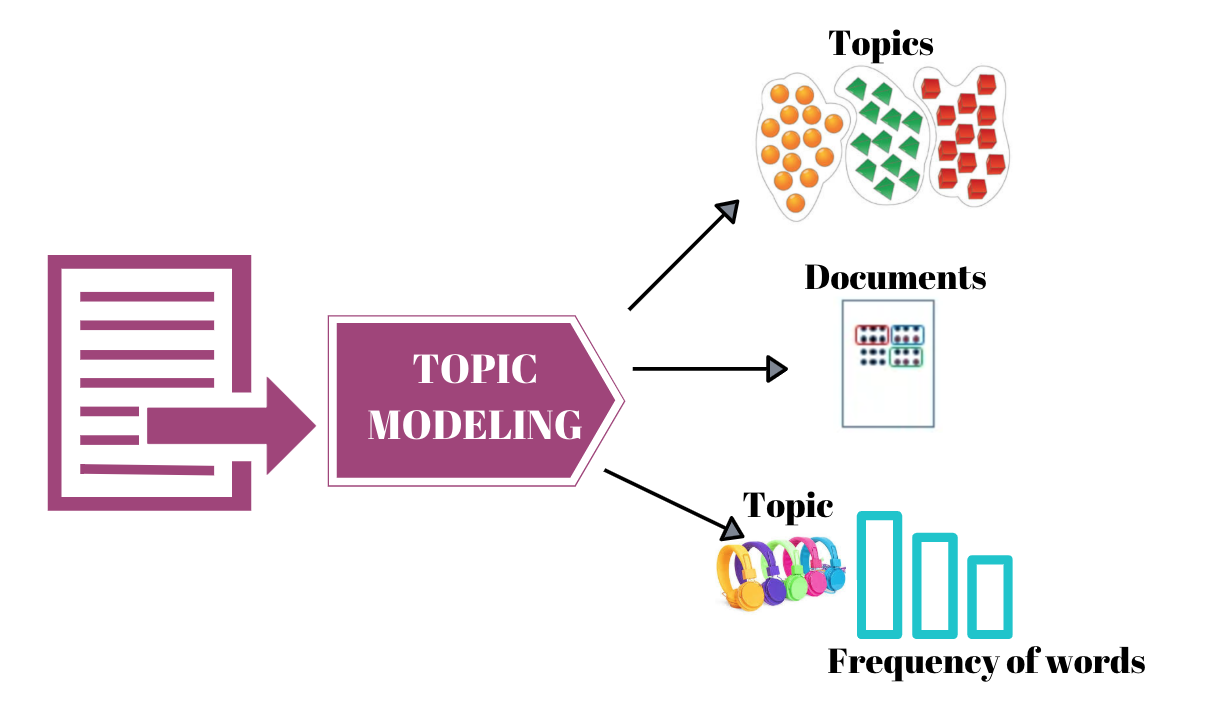
\includegraphics[width=8cm]{Graphics/topic_modeling.png}
  \end{minipage}
  \begin{minipage}{5cm}
    \textbf{Topic modeling} is often used when a large collection of text cannot be reasonably read and sorted through by a person. Topic model will discover
    \begin{itemize}
      \item Latent semantic structure.
      \item Distribution of topics.
      \item Frecuency of topics.
    \end{itemize}
  \end{minipage}

\end{frame}


\begin{frame}[fragile=singleslide]{\large \textbf{Introduction}}
  \framesubtitle{Traditional Topic Modeling Methods}
  \begin{figure}[ht!]
    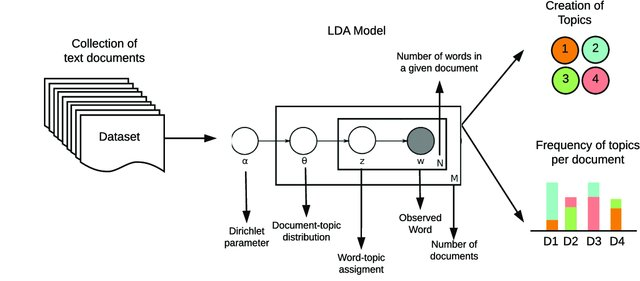
\includegraphics[width=10cm]{Graphics/LDA.jpg}
    \caption{LDA representation \cite{Buenano_Fernandez_2020}.}
  \end{figure}
\end{frame}

\begin{frame}[fragile=singleslide]{\large \textbf{Introduction}}
  \framesubtitle{Traditional Topic Modeling Methods}
  \begin{figure}[ht!]
    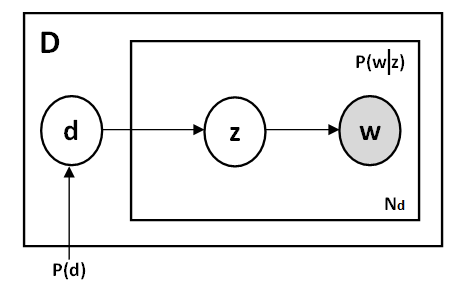
\includegraphics[width=8cm]{Graphics/plsa.png}
    \caption{PLSA representation \cite{Alghamdi_2015}.}
  \end{figure}
\end{frame}

\begin{frame}[fragile=singleslide]{\large \textbf{Introduction}}
  \framesubtitle{Distributed Representations of Words and Documents}
  \begin{figure}[ht!]
    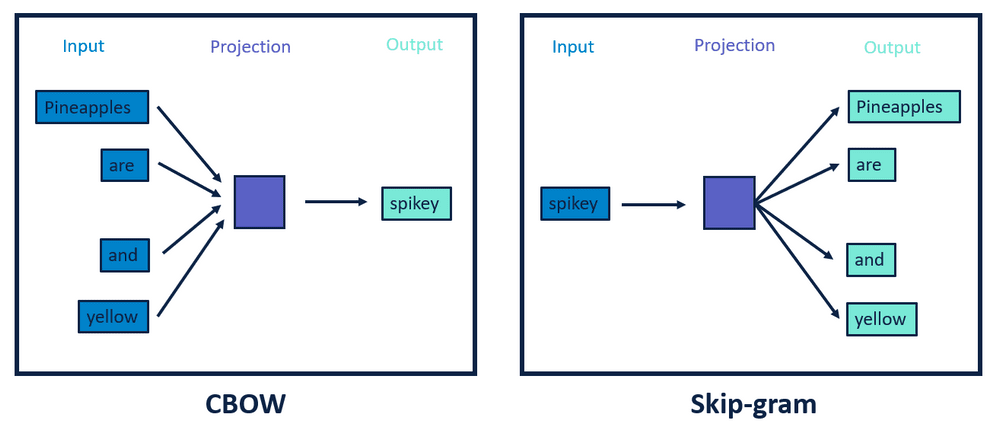
\includegraphics[width=12cm]{Graphics/word2vec.png}
    \caption{PLSA representation \cite{Alghamdi_2015}.}
  \end{figure}
\end{frame}

\begin{frame}[fragile=singleslide]{\large \textbf{Introduction}}
  \framesubtitle{Distributed Representations of Topics}
  \begin{figure}[ht!]
    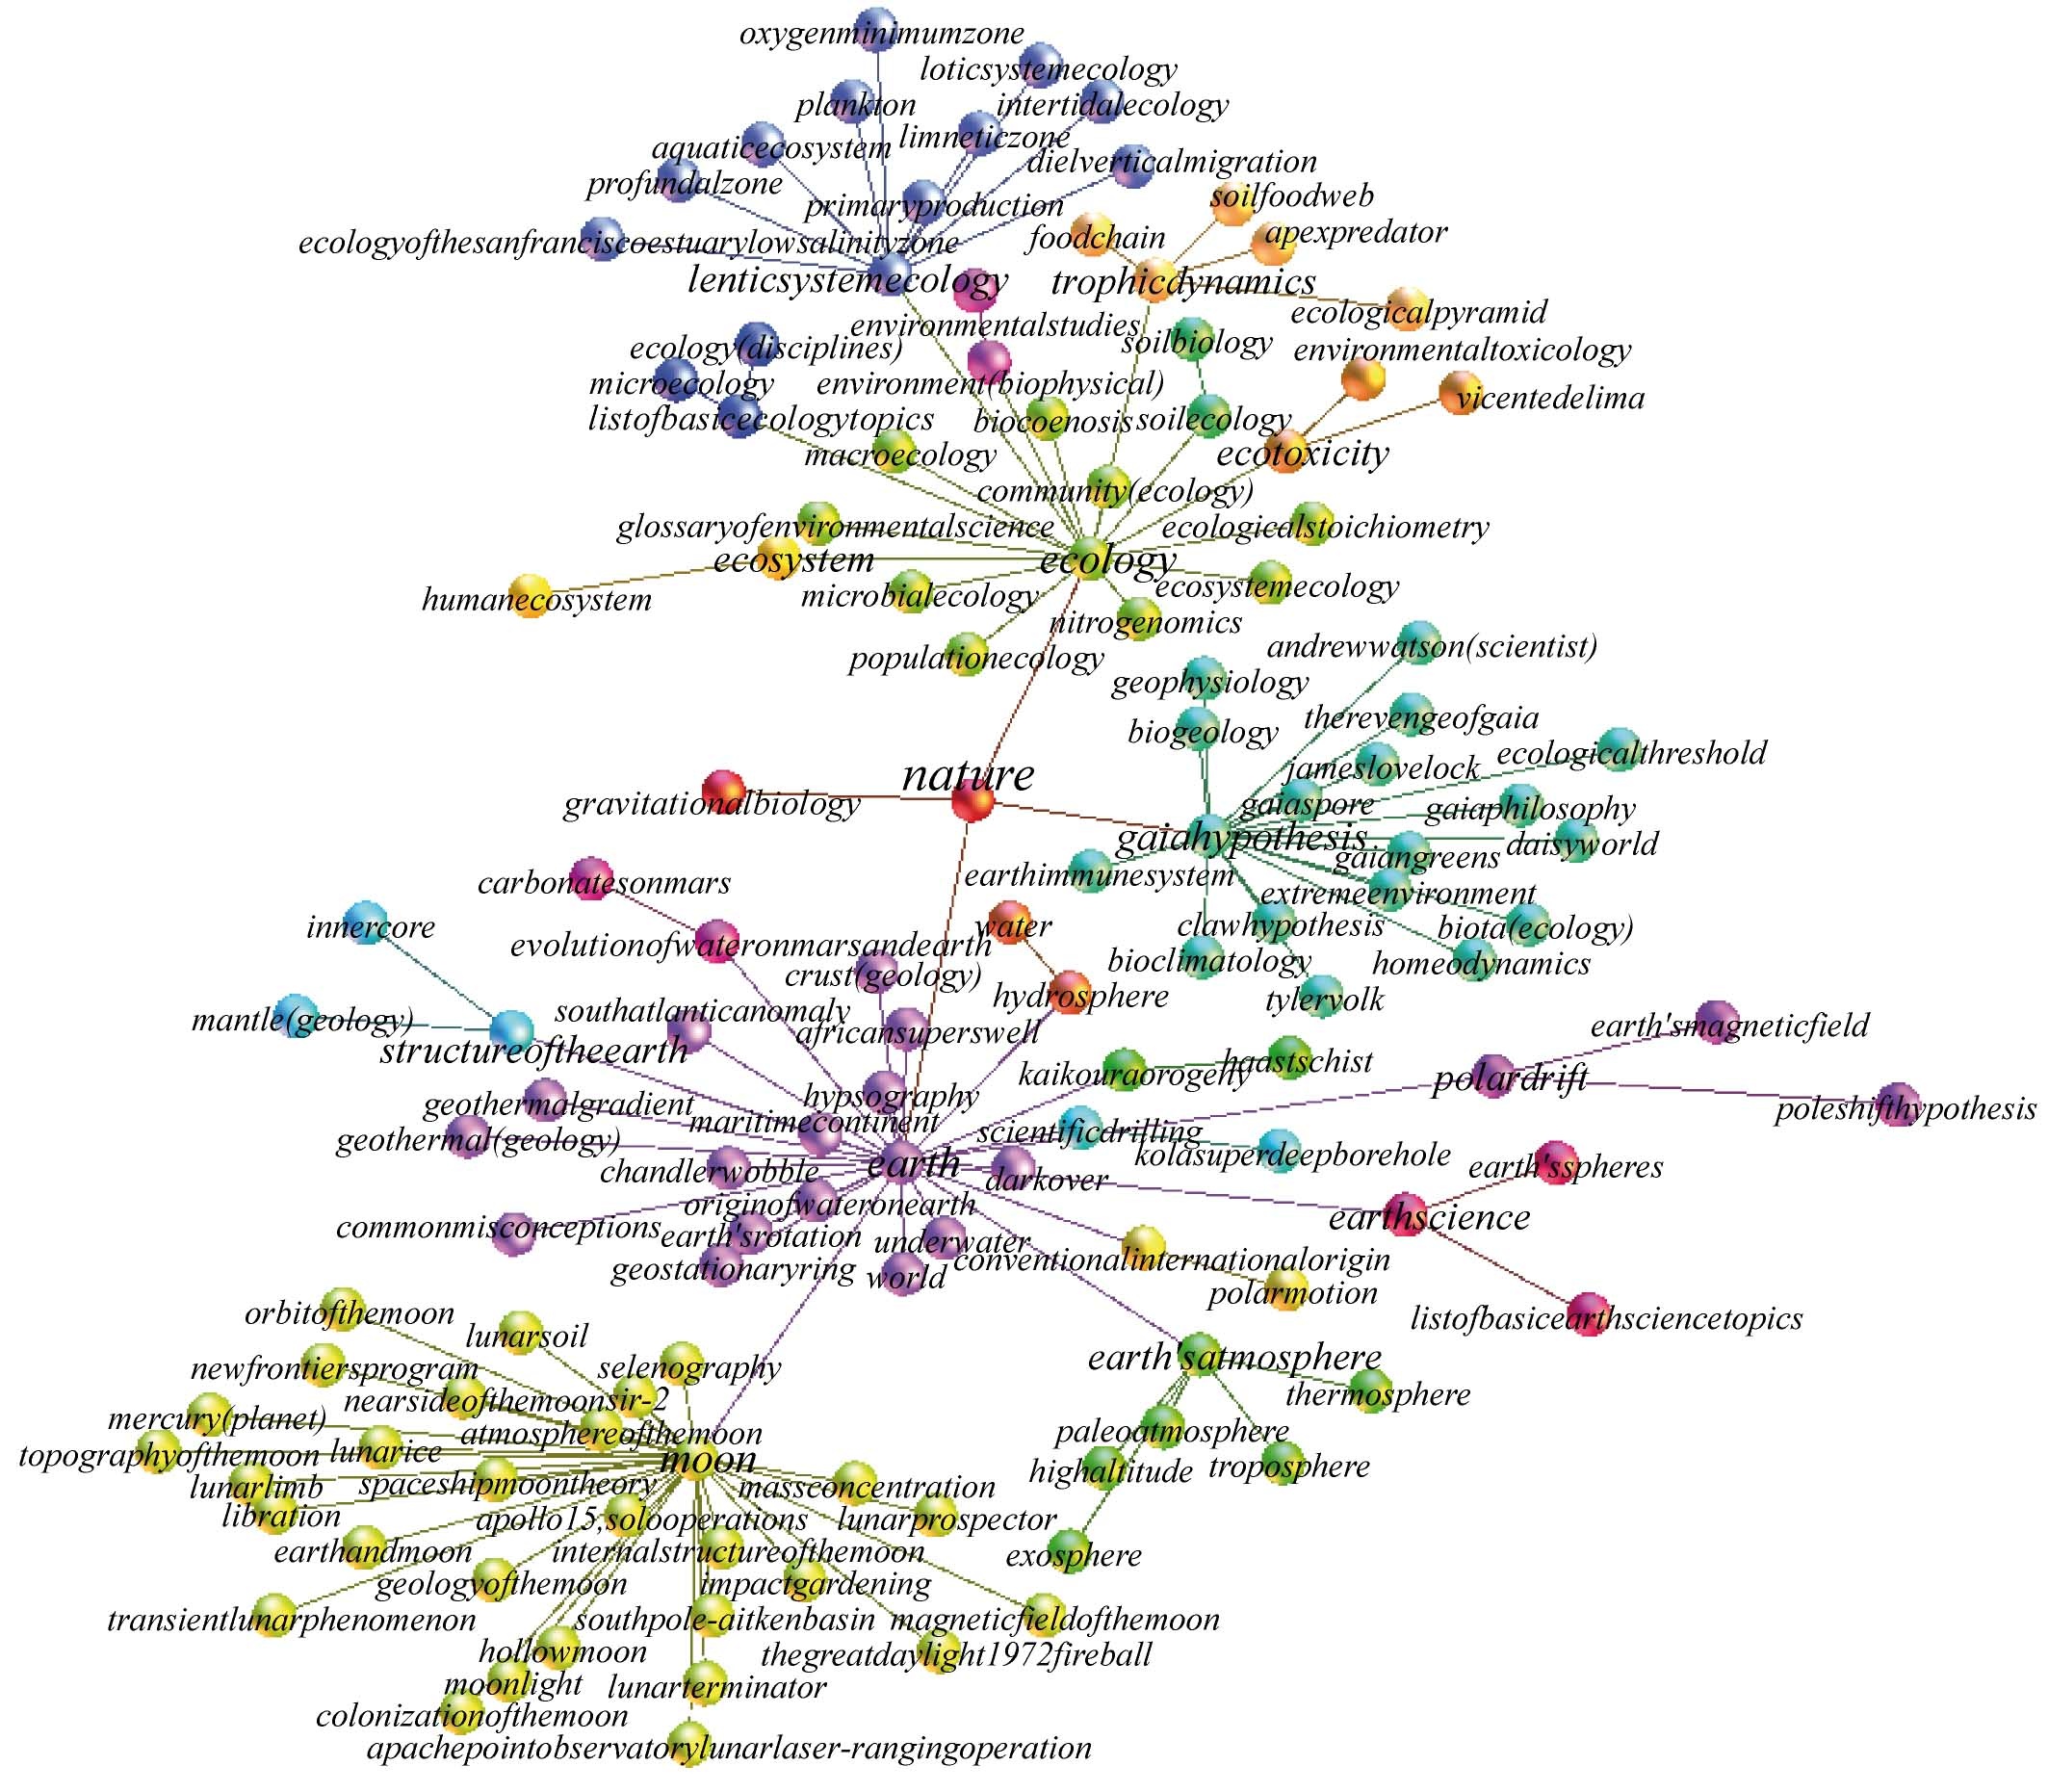
\includegraphics[width=5cm]{Graphics/semantic_space.jpg}
    \caption{semantic space \cite{Masucci_2011}.}
  \end{figure}
\end{frame}

\begin{frame}[fragile=singleslide]{\large \textbf{Model description}}
  \framesubtitle{Create Semantic Embedding}
  \begin{figure}[ht!]
    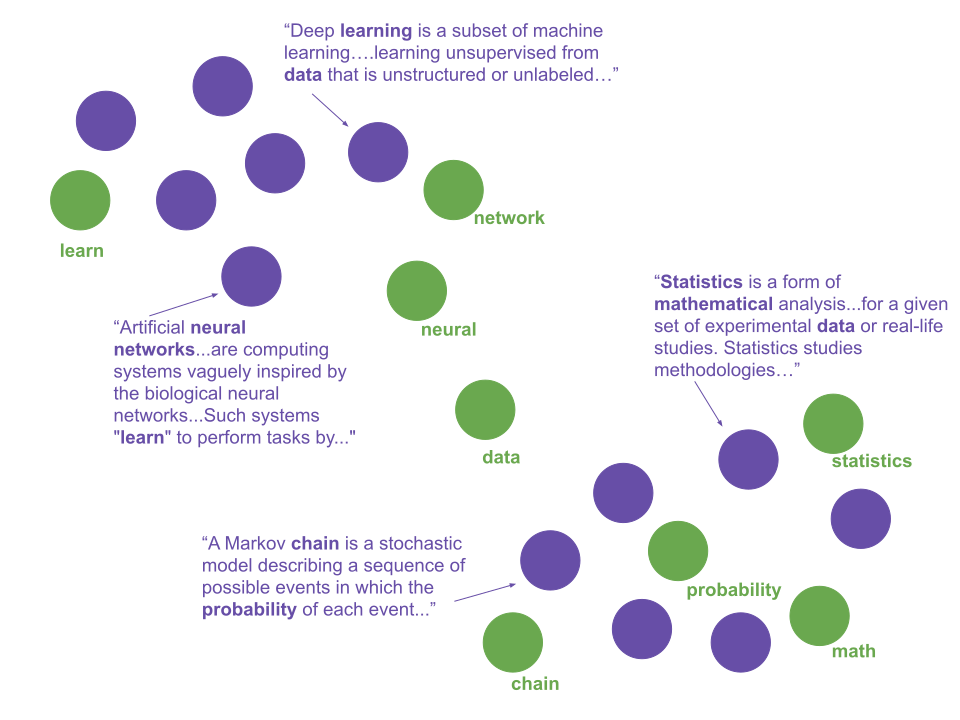
\includegraphics[width=7cm]{Graphics/doc_word_embedding.png}
    \caption{semantic space \cite{Angelov_2020}.}
  \end{figure}
\end{frame}

\begin{frame}[fragile=singleslide]{\large \textbf{Model description}}
  \framesubtitle{Find Number of Topics}
  \begin{figure}[ht!]
    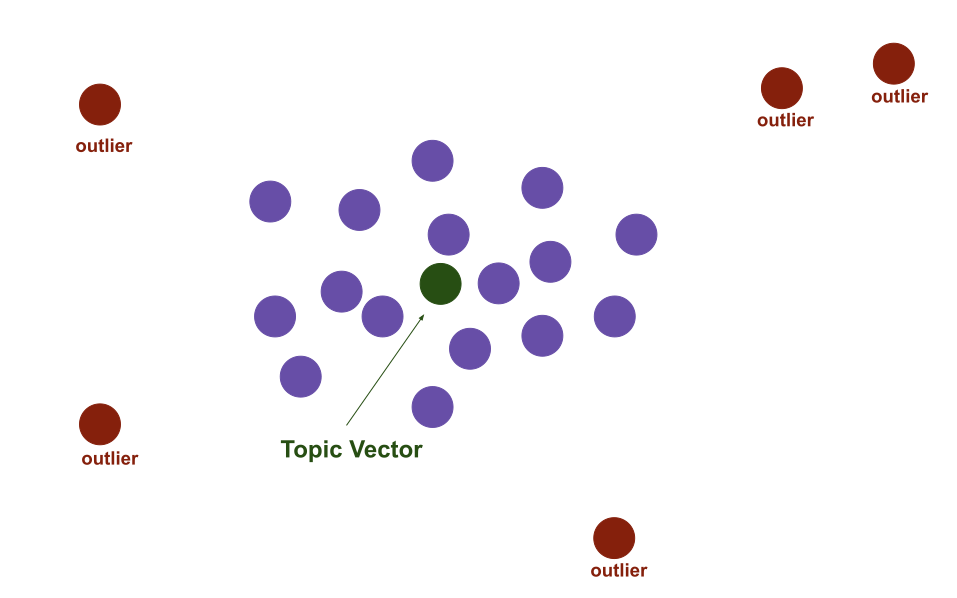
\includegraphics[width=8.5cm]{Graphics/topic_vector.png}
    \caption{Topic subspace \cite{Angelov_2020}.}
  \end{figure}
\end{frame}

\begin{frame}[fragile=singleslide]{\large \textbf{Model description}}
  \framesubtitle{Low Dimensional Document Embedding}
  \begin{figure}[ht!]
    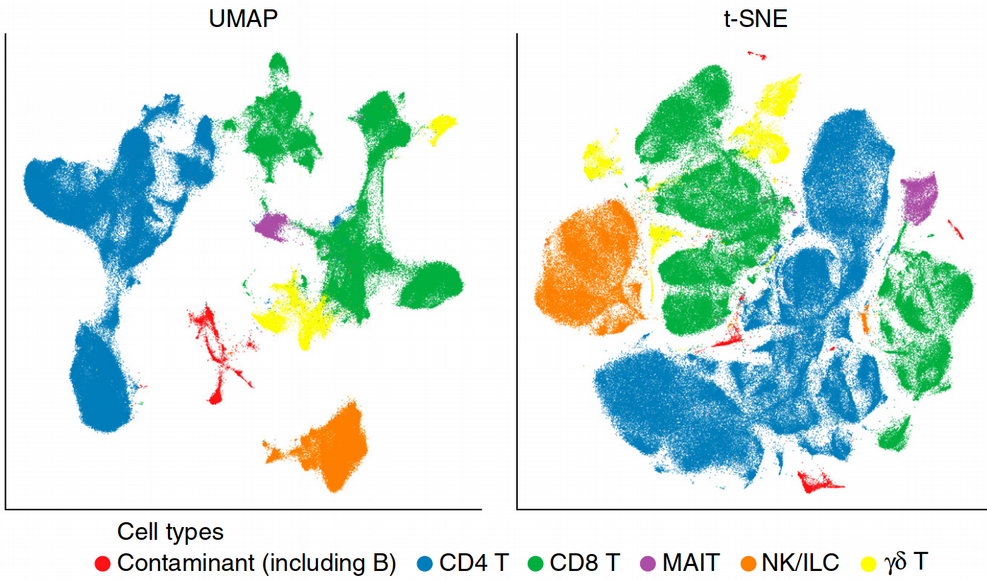
\includegraphics[width=8.5cm]{Graphics/umap.png}
    \caption{UMAP vs T-SNE \cite{Becht_2018}.}
  \end{figure}
\end{frame}

\begin{frame}[fragile=singleslide]{\large \textbf{Model description}}
  \framesubtitle{Find Dense Clusters of Documents}
  \begin{figure}[ht!]
    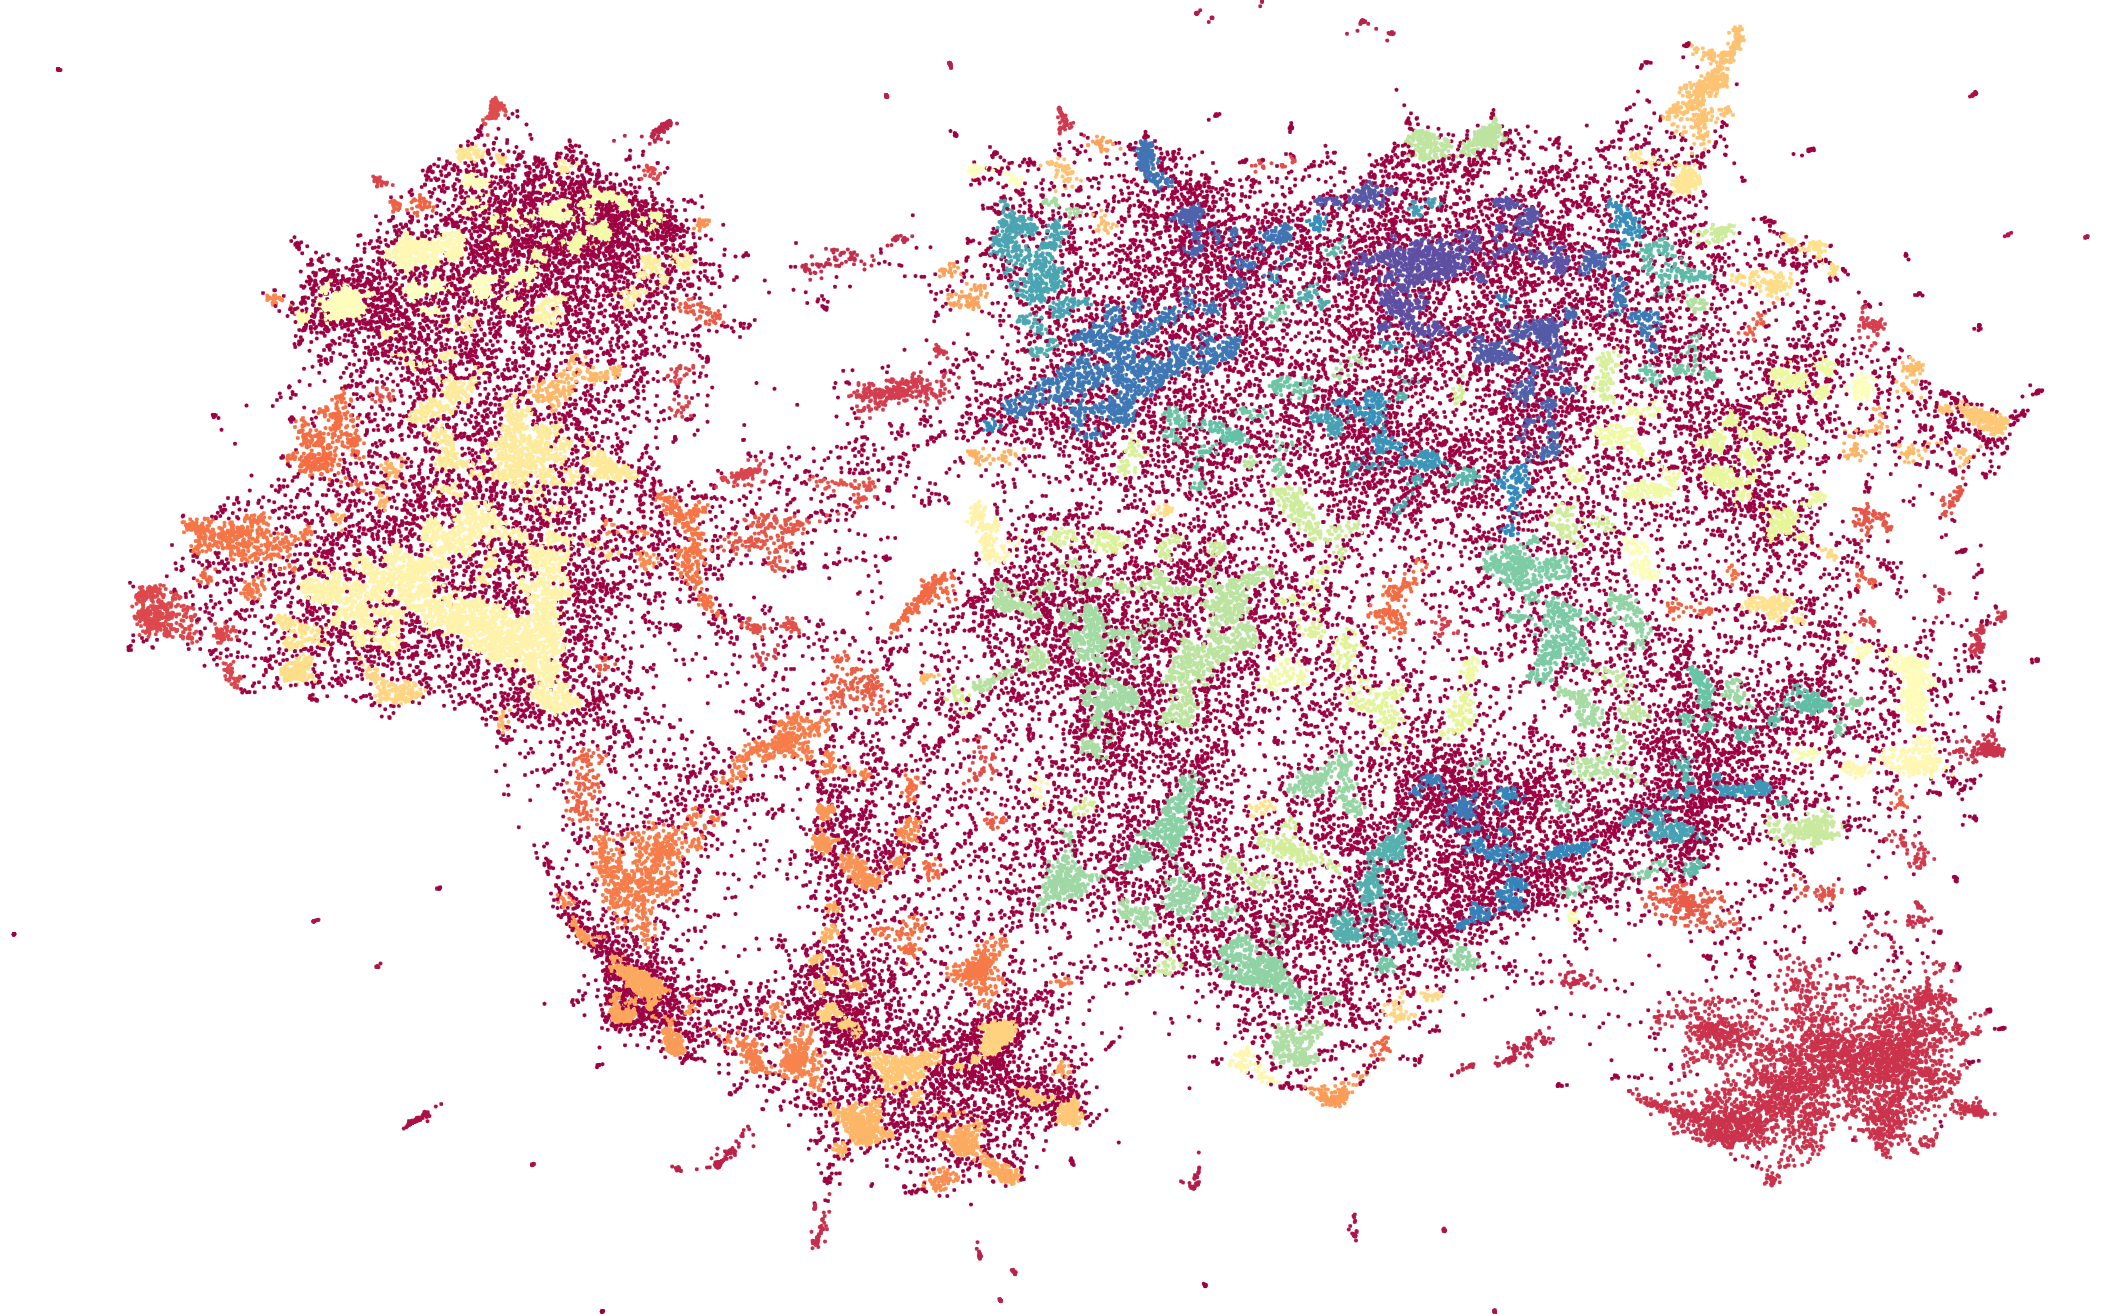
\includegraphics[width=10cm,height=5cm]{Graphics/hdbscan_docs.png}
    \caption{UMAP vs T-SNE \cite{Angelov_2020}.}
  \end{figure}
\end{frame}

\begin{frame}[fragile=singleslide]{}
  \begin{figure}[ht!]
    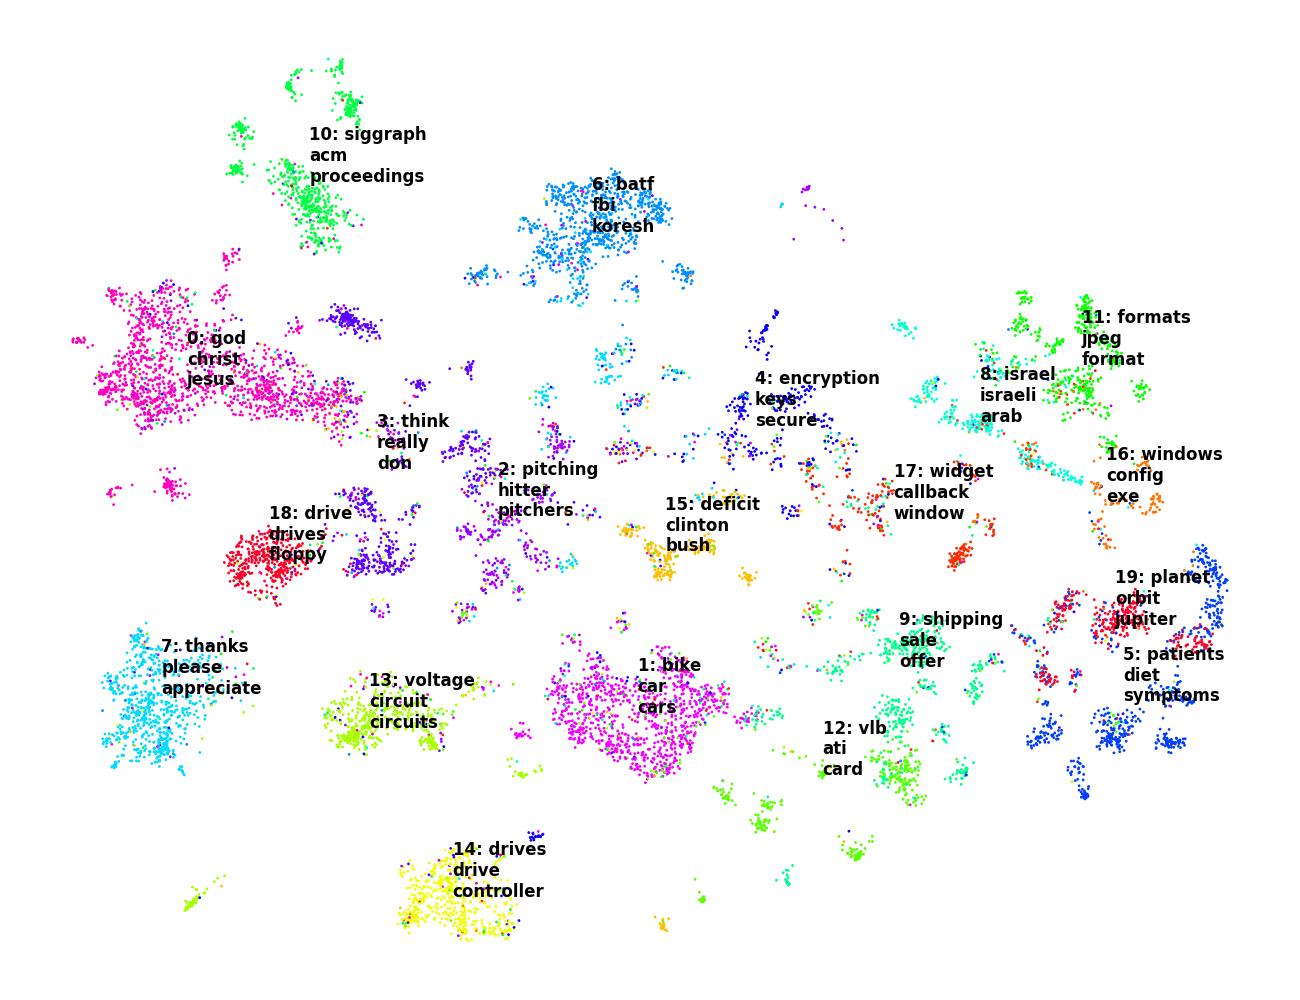
\includegraphics[height=8cm]{Graphics/news_clustered.png}
    \caption{Semantic space for 20 News Dataset.}
  \end{figure}
\end{frame}

\begin{frame}[fragile=singleslide]{}
  \begin{figure}[ht!]
    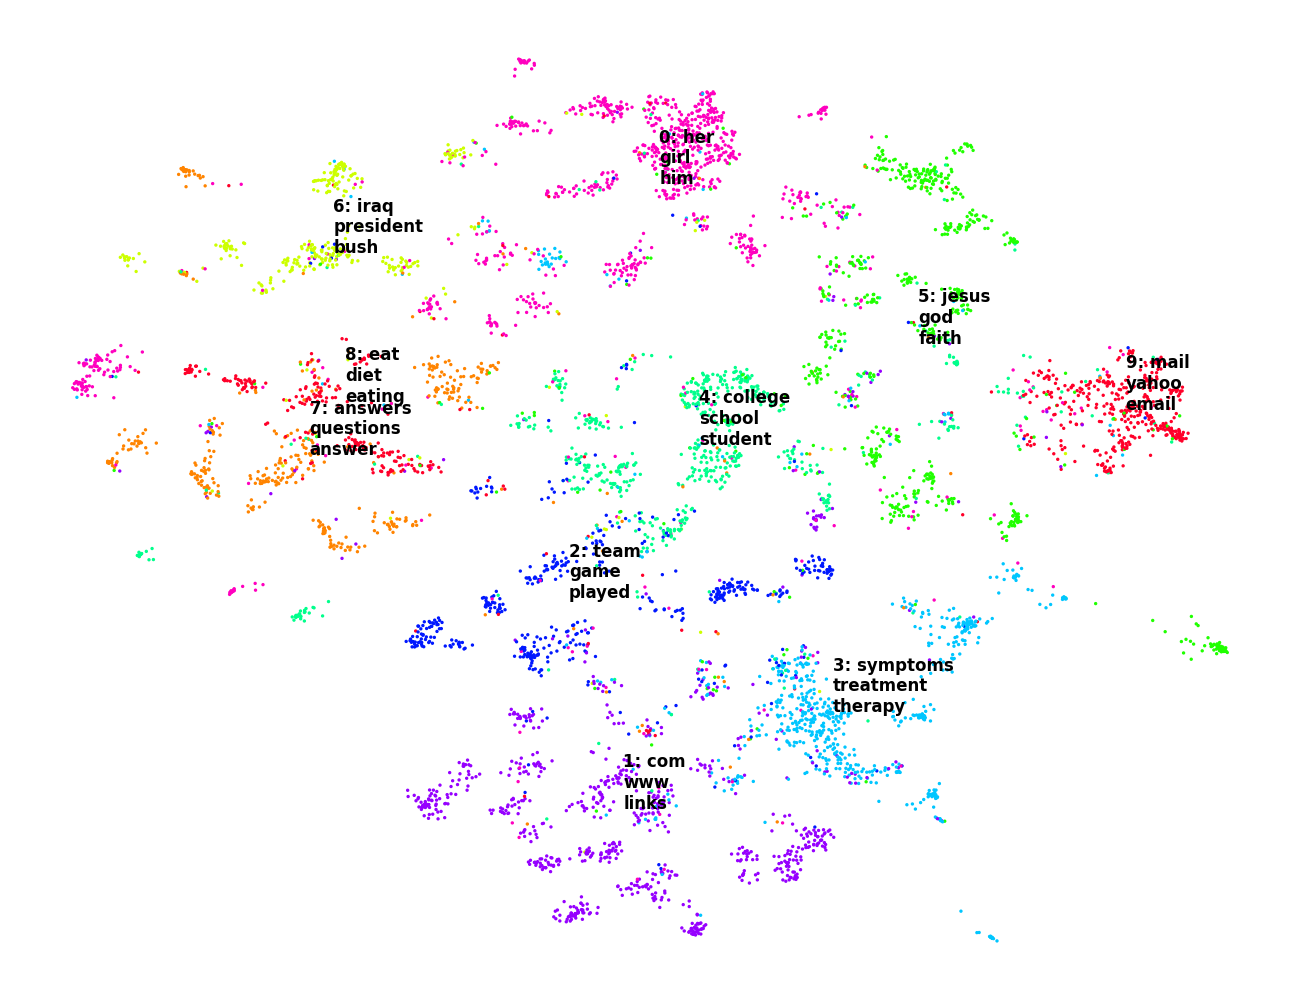
\includegraphics[height=8cm]{Graphics/yahoo_clustered.png}
    \caption{Semantic space for Yahoo Answers.}
  \end{figure}
\end{frame}

\begin{frame}[fragile=singleslide]{}
  \begin{figure}[ht!]
    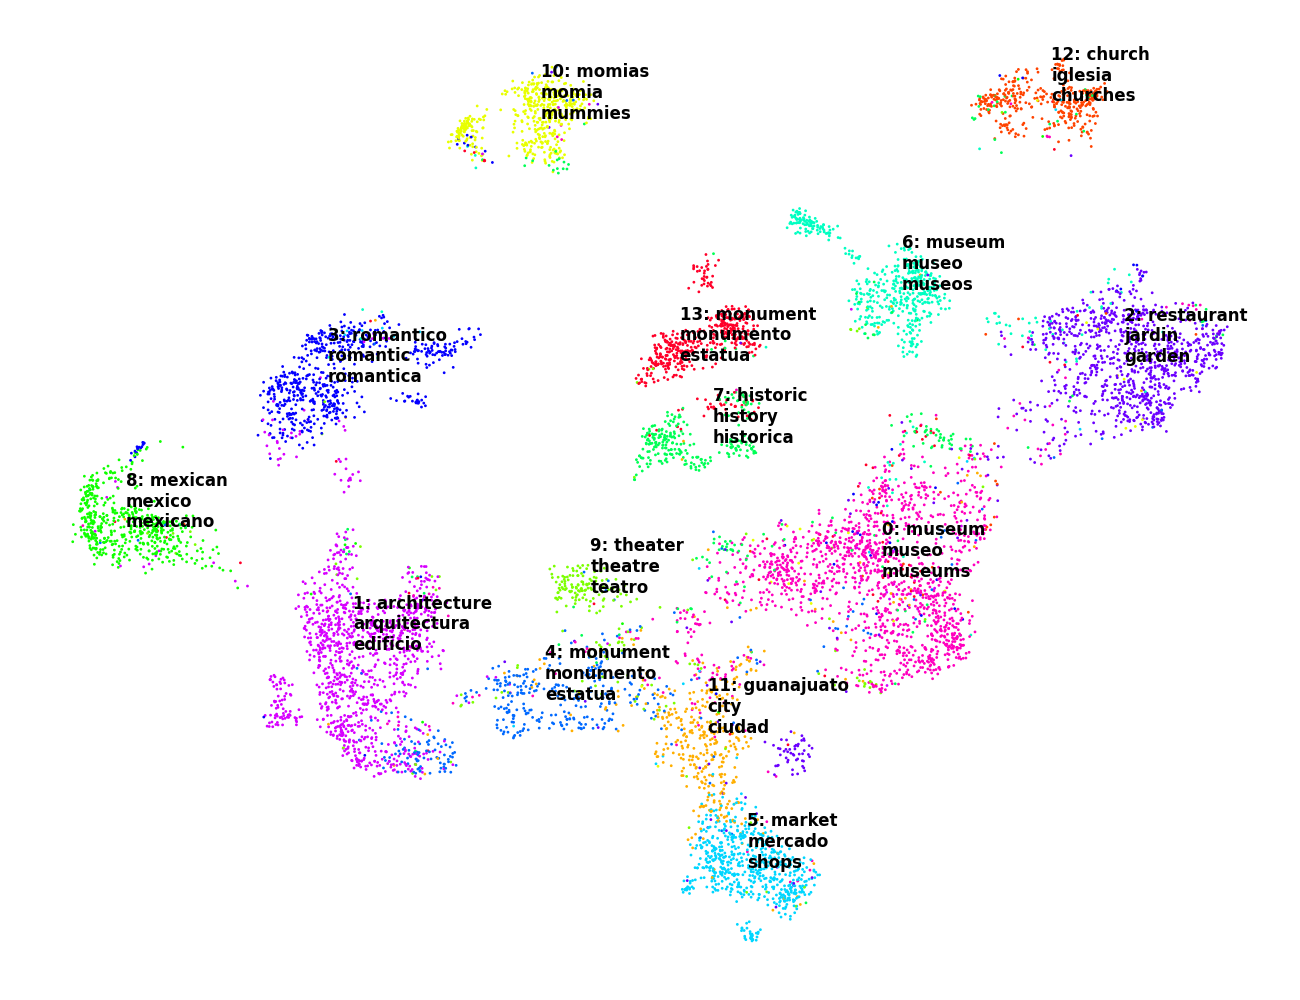
\includegraphics[height=8cm]{Graphics/tripadvisor_clustered.png}
    \caption{Semantic space for Tripadvisor.}
  \end{figure}
\end{frame}

\begin{frame}[fragile=singleslide]{\large \textbf{Code}}
  \begin{minipage}{7cm}
    \begin{figure}[ht!]
      
\includegraphics[width=7cm]{Graphics/qr.eps}
    \end{figure}
  \end{minipage}
  \begin{minipage}{7cm}
    \begin{figure}[ht!]
      
\includegraphics[width=2cm]{Graphics/github.png}\\
      \caption*{\url{https://github.com/giovannilopez9808/Natural_Language_Processing_Proyecto}}
    \end{figure}
  \end{minipage}
\end{frame}


\begin{frame}[allowframebreaks]{References}
  \bibliography{references}
  \bibliographystyle{vancouver}
\end{frame}
